% figures-es/three-statement.tex
% Standalone TikZ: vínculos del modelo de tres estados — Estado de resultados, Balance general, Estado de flujo de efectivo.
% Flechas: NI→Utilidades retenidas; D&A→CFO; CapEx→PP&E; Deuda→CFF.
\documentclass[tikz,border=6pt]{standalone}
\usepackage{tikz}
\usetikzlibrary{arrows.meta,positioning,calc}

\definecolor{vcblue}{HTML}{1A5276}
\definecolor{vcteal}{HTML}{0E6655}
\definecolor{vcgrey}{HTML}{5D6D7E}

\begin{document}
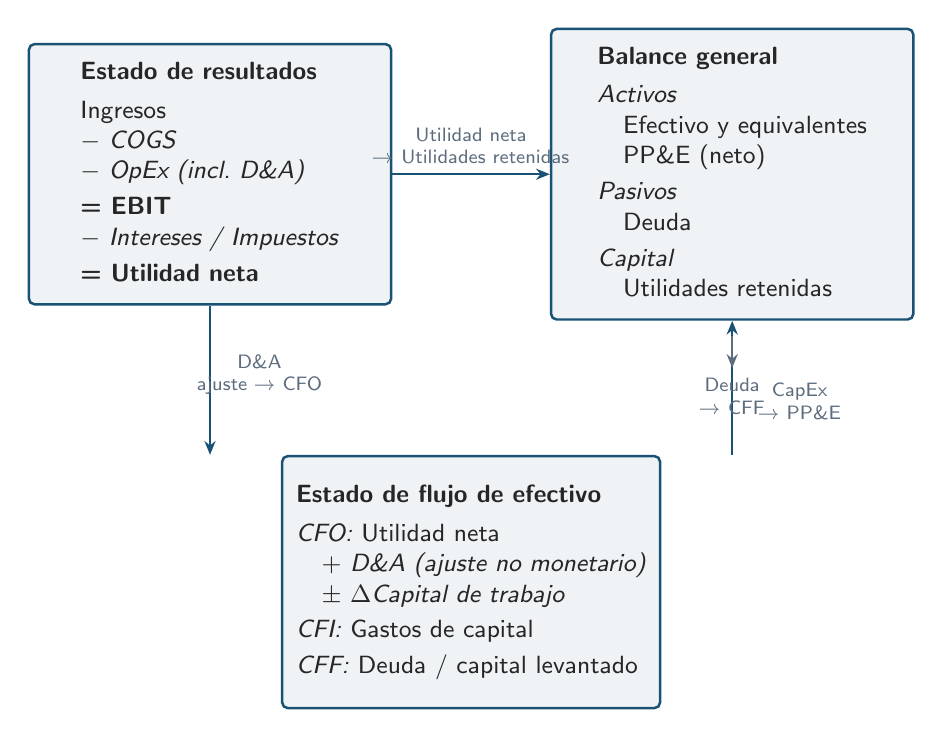
\begin{tikzpicture}[
  node distance=16mm,
  stmt/.style={draw=vcblue, line width=0.9pt, rounded corners=2pt, fill=vcblue!7,
               font=\sffamily\small, align=left,
               minimum width=46mm, minimum height=32mm, text=black!85,
               inner sep=5pt},
  hdr/.style={font=\sffamily\bfseries\small, text=vcblue},
  fld/.style={font=\sffamily\footnotesize, text=black!80},
  arrow/.style={-{Stealth[length=5pt,width=4pt]}, vcblue, line width=0.9pt},
  lbl/.style={font=\sffamily\scriptsize, text=vcgrey, align=center},
]

  %% ── Estado de resultados ──
  \node[stmt] (is) {%
    \begin{tabular}{@{}l@{}}
      \textbf{\textsf{Estado de resultados}}\\[3pt]
      Ingresos\\
      \textit{$-$ COGS}\\
      \textit{$-$ OpEx (incl.\ D\&A)}\\[2pt]
      \textbf{= EBIT}\\
      \textit{$-$ Intereses / Impuestos}\\[2pt]
      \textbf{= Utilidad neta}
    \end{tabular}};

  %% ── Balance general ──
  \node[stmt, right=20mm of is] (bs) {%
    \begin{tabular}{@{}l@{}}
      \textbf{\textsf{Balance general}}\\[3pt]
      \textit{Activos}\\
      \quad Efectivo y equivalentes\\
      \quad PP\&E (neto)\\[2pt]
      \textit{Pasivos}\\
      \quad Deuda\\[2pt]
      \textit{Capital}\\
      \quad Utilidades retenidas
    \end{tabular}};

  %% ── Estado de flujo de efectivo ──
  \node[stmt, below=18mm of $(is.south east)!0.5!(bs.south west)$] (cf) {%
    \begin{tabular}{@{}l@{}}
      \textbf{\textsf{Estado de flujo de efectivo}}\\[3pt]
      \textit{CFO:} Utilidad neta\\
      \quad \textit{$+$ D\&A (ajuste no monetario)}\\
      \quad \textit{$\pm$ $\Delta$Capital de trabajo}\\[2pt]
      \textit{CFI:} Gastos de capital\\[2pt]
      \textit{CFF:} Deuda / capital levantado
    \end{tabular}};

  %% ── Flechas con etiquetas ──

  %% Utilidad neta → Utilidades retenidas
  \draw[arrow] (is.east) -- node[above, lbl, pos=0.5] {Utilidad neta\\→ Utilidades retenidas} (bs.west);

  %% D&A → CFO (parte inferior izquierda del ER a parte superior izquierda del EFE)
  \draw[arrow] (is.south) -- ++(0,-6mm)
    node[lbl, below right, yshift=1mm, xshift=-3mm] {D\&A\\ajuste → CFO}
    -- (cf.north -| is.south);

  %% CapEx → PP&E (parte superior derecha del EFE a parte inferior derecha del BG)
  \draw[arrow] (cf.north -| bs.south) -- (bs.south)
    node[lbl, right, pos=0.4, xshift=2mm] {CapEx\\→ PP\&E};

  %% Deuda → CFF anotación (dentro del EFE, nota autorreferencial)
  \draw[arrow, vcgrey] (bs.south) ++(0,-2mm) -- ++(0,-4mm)
    node[lbl, below, vcgrey] {Deuda\\→ CFF};

\end{tikzpicture}
\end{document}
